\capitulo{5}{Aspectos relevantes del desarrollo del proyecto}

En este apartado se recogen los aspectos más interesantes del desarrollo del proyecto que se han detectado 
durante las fases de Análisis, Diseño e Implementación. Se incluye también un apartado con un workflow que sirve
de ejemplo de uso de los nodos desarrollados. 

\section{Análisis}

Como resultado de la fase de Análisis se han completado los apartados: 

\begin{itemize}
	\item Plan de proyecto Software (Apéndice A)
	\item Especificación de requisitos (Apéndice B)
\end{itemize}

Durante la fase de análisis se realiza un estudio previo para determinar el alcance del proyecto y 
las posibilidades y limitaciones de las herramientas y tecnologías involucradas. También se instala el entorno
de trabajo completo y se realizan las pruebas técnicas necesarias para asegurar que se podrán cumplir los objetivos
del proyecto. Concretamente, se abordan las siguientes cuestiones: 

\begin{itemize}
	\item Extracción de datos de Moodle. Pruebas de acceso a la API de Moodle y los diferentes logs disponibles. 
    \item Estudio previo del desarrollo en KNIME, incluyendo también la implementación de nodo KNIME de prueba y
	 creación de un workflow para ejecutar el nodo desarrollado en combinación con otros nodos del núcleo de KNIME.
	\item Elección de los datos de estudio y workflow a implementar.  
\end{itemize}


\subsection{Extracción de datos de Moodle}

Se realiza un primer estudio de los métodos de acceso a los datos de Moodle. Aunque Moodle tiene una REST API muy completa para acceder a diferente tipo de información a través de servicios 
web, en este punto se detecta que los servicios web de Moodle no ofrecen acceso a todos los
datos que se pueden visualizar desde Moodle. 
\

Buscando métodos de acceso alternativos a Moodle, se localiza la aplicación UBUMonitor, un proyecto desarrollado 
en Java que sí extrae de Moodle todos los logs que nos gustaría incorporar en nuestro proyecto. El código de UBUMonitor 
nos aporta dos soluciones importantes: 

\begin{itemize}
	\item Código de acceso a Moodle mediante Web Scrapping, simulando el acceso como si se tratara de un login realizado en el sitio web Moodle. 
	\item Código de acceso a los logs.
\end{itemize}

Se decide incorporar directamente a nuestro proyecto las clases relevantes de UBUMonitor, generando el archivo JAR que nos
permite importar el código al proyecto. 
\

En resumen, como solución adoptada, se realizará un \textbf{doble login en Moodle}. El primer login se realiza siguiendo el modelo de webservice de la APP de Moodle. Esto 
implica que \textbf{la plataforma Moodle debe tener activa la opción de acceso a la APP de Moodle}. El segundo login se realiza
a través de Web Scrapping con las clases aportadas por UBUMonitor. Este doble acceso es transparente para el usuario. 

\subsubsection{Género del usuario}

Moodle no almacena información de género del usuario. Para poder realizar estudios teniendo en cuenta el género, se ha 
utilizado el servicio externo \href{https://genderize.io/}{genderize.io}, que nos indica, a través de su API, el género de una 
persona a partir de su nombre (male o female). 


\subsubsection{Anonimización}

Se desea que el profesor que extrae los datos de Moodle pueda tener la información de los usuarios sin anonimizar, ya que los 
estudios que realice pueden ir orientados a la gestión directa de su acción formativa, lo que requeriría conocer el nombre
de los alumnos afectados. 
\

Sin embargo, también se quiere aportar la posibilidad de que el profesor utilice sus datos o resultados para sus 
proyectos o artículos de investigación, por lo que se quiere facilitar cierto grado de anonimización. Se incorpora al proyecto
una anonimización sencilla cambiando el nombre y apellidos del usuario con el servicio \href{https://www.datafaker.net/}{Data Faker}. Primero se obtiene el 
género del usuario y posteriormente se genera un nombre falso apropiado para ese género. 
\

Por complejidad, se escapa del alcance de este proyecto un sistema más seguro de anonimización de los datos, que ofusque 
también la información relacionada con el usuario como, por ejemplo, su ID. En cualquier caso, KNIME dispone de funcionalidades
adicionales de anonimización que se podrían incorporar como parte del flujo de trabajo. 


\subsection{Estudio previo del desarrollo en Knime}

\subsubsection{Pasos para crear una extensión y nodo de ejemplo en KNIME}

Los nodos de KNIME son elementos que aportan una funcionalidad independiente. Estos nodos se pueden combinar dentro de un 
flujo de trabajo o workflow para realizar funciones más complejas. Los nodos vienen empaquetados dentro de extensiones de KNIME, que 
pueden incluir uno o varios nodos relacionados. 
\

Los pasos para crear una extensión en KNIME se pueden resumir en: 

\begin{enumerate}
	\item Montar el entorno de desarrollo con KNIME SDK y Eclipse.
	\item Crear un nuevo proyecto de tipo KNIME Extension. 
	\item Implementar la extensión. 
	\item Probar la extensión. 
	\item Desplegar la extensión. 
\end{enumerate}

KNIME nos facilita una \href{https://docs.knime.com/latest/analytics_platform_new_node_quickstart_guide/index.html#_introduction}{guía 
para desarrollar en Java una extensión con un primer nodo de ejemplo}, llamado \textbf{Number Formatter}. Este nodo recibe como entrada 
una tabla de datos con una columna con números decimales, y devuelve una tabla similar con los datos redondeados al número 
de decimales especificados en la configuración del nodo. 
\

En este punto se estudia el código generado por KNIME para este nodo de ejemplo, además de otros nodos de ejemplo similares 
a los que queremos desarrollar. 


\subsubsection{Reutilización de nodos en KNIME a nivel de código}

Durante la fase de Análisis se realizan pruebas para verificar si un nodo de KNIME puede ejecutarse a nivel de código desde 
dentro de otro nodo. Esto podría ser interesante para reutilizar ciertas funcionalidades que están disponibles en KNIME 
a través de nodos, como puede ser conversión de datos de unos tipos a otros. 
\

Aunque se podría pensar que es posible embeber o reutilizar la funcionalidad de un nodo desde programación como si 
se tratara de una función (parámetros de entrada) y recuperar la salida, se descubre que los nodos no se pueden ejecutar a nivel de código. Esto es, no podemos inyectar la funcionalidad completa de un nodo 
dentro de otro, ejecutándolo internamente. Se confirma a partir de comunicaciones con miembros del equipo de KNIME, que se ha 
impuesto esta restricción de diseño para evitar la alta dependencia entre nodos y los problemas que ello conllevaría a nivel 
de mantenimiento cuando un nodo queda obsoleto. Se puede consultar \href{https://forum.knime.com/t/using-node-without-gui/2044/8}{este hilo del foro de soporte de KNIME} donde se confirma esta restricción impuesta en el desarrollo. 
\

\subsubsection{Estudio de otros nodos}

Las extensiones de KNIME están disponibles con código abierto. De entre las extensiones disponibles en KNIME Community Hub, la extensión 
\href{https://hub.knime.com/knime/extensions/org.knime.features.ext.twitter/latest}{KNIME Twitter Connectors} dispone de un 
conjunto de nodos con una funcionalidad parecida a la que queremos implementar, por lo que se revisa el código de implementación
como guía para nuestra implementación. En general, para futuros desarrolladores de KNIME, se aconseja seguir este procedimiento, 
localizando nodos de funcionalidad o estructura similar a la que se quiera desarrollar. 

\subsubsection{Reutilización de librerías externas}

Al tratarse de un proyecto Java, se pueden importar en el proyecto librerías externas en formato JAR. Las aplicaciones UBUMonitor y Datafaker 
han sido importadas por esta vía. 


\subsection{Datos de estudio y workflows a implementar}

Durante el análisis se evalúan las posibles fuentes de datos y posibles workflows de trabajo. Para el desarrollo se pueden 
utilizar los datos de prueba disponibles en la \href{https://school.moodledemo.net/}{demo de Moodle Mount Orange School}, que es un 
Moodle ya montado con cursos, actividades y usuarios. 
\

Se decide implementar un único workflow sobre datos reales que utilice diferentes técnicas de Aprendizaje Supervisado. 

\newpage
\section{Diseño}

Como resultado de la fase de Diseño se ha completado la Especificación de diseño, que se puede consultar en el Apéndice C de esta memoria. 

\subsection{Aspectos relevantes del diseño}

A la hora de decidir el Diseño de la extensión y tipos de nodos que incluirá, se evalúan las siguientes estrategias: 

\begin{enumerate}
	\item Crear nodos individuales por cada web service de Moodle o pieza de información a extraer. Por ejemplo, un nodo 
	para extraer los logs de participación en foros, otro nodo para extraer los logs de consulta de actividades, etc. 
	\item Crear nodos más genéricos que extraen información de varios web services relacionados. Por ejemplo, 
	un nodo para extraer toda la información de usuarios, otro para cursos, otro para logs, etc. 
\end{enumerate}

Se opta por la segunda opción y se plantea el diseño de estos 6 nodos: 

\begin{itemize}
	\item \textbf{Moodle Connector}. Establece la conexión con la plataforma. 
	\item \textbf{Moodle Courses}. Devuelve información de cursos disponibles en la plataforma. 
	\item \textbf{Moodle Users}. Devuelve el listado de usuarios matriculados en los cursos especificados. 
	\item \textbf{Moodle Reports Logs}. Devuelve un amplio abanico de logs de interacción de los usuarios disponibles en Moodle. 
	\item \textbf{Moodle Reports Grades}. Devuelve calificaciones de los alumnos en las actividades indicadas. 
	\item \textbf{Moodle Reports Quizzes}. Devuelve información relacionada con los cuestionarios realizados por los alumnos. 
\end{itemize}


\newpage
\section{Implementación}

Como resultado de la fase de Implementación se han completado los apartados: 

\begin{itemize}
	\item Documentación técnica de programación (Apéndice D)
	\item Documentación de usuario (Apéndice E)
\end{itemize}


\subsection{Problemas encontrados durante la implementación}

Se destacan en este apartado algunos de los problemas más relevantes encontrados durante la implementación de la extensión. 


\subsubsection{Versión de KNIME}

El desarrolló del proyecto comenzó en la versión KNIME 4.5.2. Durante el desarrollo se lanzó la versión 4.7 
y se actualizó el código y el entorno de desarrollo para que la extensión desarrollara fuera compatible con 
esta versión. 

Antes de la entrega del proyecto se ha publicado una nueva versión de KNIME, 5.1, que no es del todo compatible 
con los nodos anteriores y la extensión desarrollada no se ha actualizado a esta versión. Sí que se ha comprobado que 
sigue siendo compatible con la última versión 4.7.x lanzada, que es la versión 4.7.7 (agosto 2023).

\subsubsection{Entorno de desarrollo}

En el apéndice D se describen los pasos requeridos para montar en entorno de desarrollo. 

Como apunte, es importante establecer una versión fija de KNIME en Target definition para descargar los plugins 
correspondientes. Por defecto KNIME establece la versión ``nightly'', con lo que el entorno se irá actualizando automáticamente a la última versión disponible. 
Esto podría, ocasionalmente, ``romper'' nuestro entorno de trabajo al producirse un salto de versión mayor (por ejemplo, de 4.6 a 4.7, de 5.1 a 5.2, etc.). 
Como ya hemos comentado, nosotros trabajaremos en la versión 4.7.7.


\subsubsection{Integración de librerías externas}

Ha sido necesario incorporar algunos proyectos externos, como:

\begin{itemize}
	\item \href{https://github.com/yjx0003/UBUMonitor/releases}{UBUMonitor 2.10.2 (20220426)}
	\item \href{https://www.datafaker.net/releases/1.7.0/}{Datafaker 1.7}
	\item \href{https://github.com/stleary/JSON-java}{JSON in Java (20220320)}
\end{itemize}

Se puede consultar el listado completo de librerías externas en la carpeta /libraries de la extensión. 
\

Inicialmente se intentaron utilizar directamente las clases de logs de UBUMonitor, pero se 
encuentraron problemas de dependencias que obligaron a extraer las clases directamente a nuestro proyecto. 
La base del código es similar pero se ha modificado posteriormente para adaptar el código a los logs específicos que se incorporaron al proyecto. 

\subsubsection{Login de Moodle}

Como ya se comentó previamente, el acceso a los datos de Moodle está limitado, por lo que se ha tenido que utilizar 
un doble acceso vía webservice similar al utilizado por la APP de Moodle, combinado con el acceso por Web Scrapping aportado 
por UBUMonitor. Esto implica que la implementación de Moodle debe tener activa la opción de acceso de la APP, algo que ya es muy 
habitual en las plataformas universitarias. 


\subsubsection{Despliegue de la extensión desarrollada}

En la \href{https://docs.knime.com/latest/analytics_platform_new_node_quickstart_guide/index.html#_deploy_your_extension}{guía para crear extensiones de KNIME en Java (apartado Deploy your extension)}, se explican dos métodos para desplegar la extensión 
desarrollada de forma que pueda ser importada en cualquier instancia de KNIME sin necesidad de integración
con Eclipse: 

\begin{itemize}
	\item \textbf{Opción 1. Sitio de actualización local  (Local Update Site)}. Esta es la opción recomendada y la que hemos 
	seguido en este proyecto. Se crea a partir de la extensión
	desarrollada una "feature" que se añade a un sitio de actualización local. La carpeta generada, que se ha compartido 
	en el repositorio del proyecto, se puede utilizar para importar el plugin desde cualquier instancia de KNIME. Las instrucciones de 
	instalación se pueden consultar en el Manual de usuario de esta memoria (apéndice E). 
	\item \textbf{Opción 2. dropin}. Se trata de exportar la extensión en formato JAR y añadirla en la carpeta "dropin" 
	de la instalación de KNIME. Aunque no está correctamente documentado, esta opción dejó de funcionar en la versión KNIME 4.1 y 
	se recuperó posteriormente en la versión 4.2. Sin embargo, nunca ha sido un método recomendado porque Eclipse tenía intención de eliminarlo. 
	\textbf{En las últimas versiones de KNIME probadas (4.5 y 4.7) esta funcionalidad parece no estar disponible}. 
\end{itemize}


\newpage
\section{Workflow de KNIME con datos reales}

A continuación presentamos un estudio práctico utilizando la extensión desarrollada dentro 
de un workflow de KNIME aplicado al Aprendizaje Supervisado. 

\subsection{Datos de estudio}

Los datos se corresponden con copias de seguridad de Moodle de la asignatura ``Aprendizaje no supervisado'' que se imparte en este Máster dentro del bloque de Ciencia de Datos. 
Concretamente se disponen de los datos correspondientes a los cursos 2021/2022 y 2022/2023. Las copias de seguridad son completas, por lo que incluyen todas las interacciones de los alumnos y sus calificaciones parciales y finales. 
Aunque se disponía también de los datos del curso 2018/2019, finalmente se descartaron porque el curso había cambiado significativamente a nivel estructural, y las actividades y su evaluación no se correspondían con los datos de años posteriores. 
\

Los datos se han importado en una instancia de Moodle local para su acceso desde Knime con el rol de Profesor. 
\

En total disponemos de registros de 56 estudiantes, 26 matriculados en el curso de 2021/2022 y 30 en el de 2022/2023. 

\subsection{Objetivo del estudio}

Para entender el siguiente estudio necesitamos conocer la metodología de estudio y evaluación utilizada dentro de la asignatura ``Aprendizaje no supervisado''. 
\

La asignatura se divide en cuatro unidades (UD1, UD2, UD3 y UD4), con evaluación teórica y práctica. La evaluación teórica consiste
en un cuestionario final por bloque (C1, C2, C3 y C4), donde el estudiante tiene un máximo de 3 intentos limitados en tiempo. 
La calificación final de cada cuestionario será la calificación máxima obtenida en los intentos realizados. 
\

Para preparar estos cuestionarios finales, en cada unidad se dispone de una serie de documentos en PDF y Vídeos con \textbf{cuestionarios de autoevaluación} asociados. 
Estos cuestionarios de autoevaluación no computan para la calificación final y tienen intentos ilimitados. Cada cuestionario solo está disponible cuando se 
completa y supera el cuestionario inmediatamente anterior, según la calificación mínima requerida en cada cuestionario. Si el estudiante desea mejorar el resultado, incluso si 
el cuestionario ya está superado, puede volver a visualizar el vídeo correspondiente y realizar nuevamente el cuestionario. Hay que recalcar que tanto la visualización de 
los vídeos como la realización de los cuestionarios de autoevaluación es opcional. 
\

Para este estudio se desea implementar un \textbf{modelo que sea capaz de predecir la calificación final en los cuestionarios de evaluación (Suspendido, Aprobado, Notable o Sobresaliente), 
a partir de información de interacción de los usuarios con los recursos de la plataforma y de los resultados obtenidos en los cuestionarios de autoevaluación}. 
Concretamente extraeremos los siguientes campos: 

\begin{itemize}
	\item \textbf{videosviews}. Número total de visualizaciones de vídeos.
	\item \textbf{courseviews}. Número total de visualizaciones de recursos del curso.
	\item \textbf{forumcount}. Número total de visualizaciones de mensajes del foro. 
	\item \textbf{autoevaltotalattempts}. Número total de intentos en cuestionarios de autoevaluación. 
	\item \textbf{autoevalgrademean}. Calificación media obtenida en los cuestionarios de autoevaluación.
\end{itemize}

Siendo la clase a predecir: 

\begin{itemize}
	\item \textbf{evalgradecategory}. Calificación final obtenida en los cuestionarios de evaluación (Suspendido, Aprobado, Notable, Sobresaliente). 
\end{itemize}


\subsection{Recopilación, limpieza y preparación de los datos}

En la Figura ~\ref{fig:workflow0} se muestra la parte del workflow relativa a la recopilación, limpieza y preparación de los datos. De la extensión desarrollada en 
este proyecto, necesitamos los nodos Moodle Connector, Moodle Users, Moodle Reports Logs y Moodle Reports Quizzes. Para este caso de estudio no 
será necesario el nodo Moodle Reports Grades, ya que las calificaciones que necesitamos están relacionadas con cuestionarios y ya están disponibles a través del nodo Moodle Reports Quizzes. 

\begin{figure}[!htb]
	\centering
	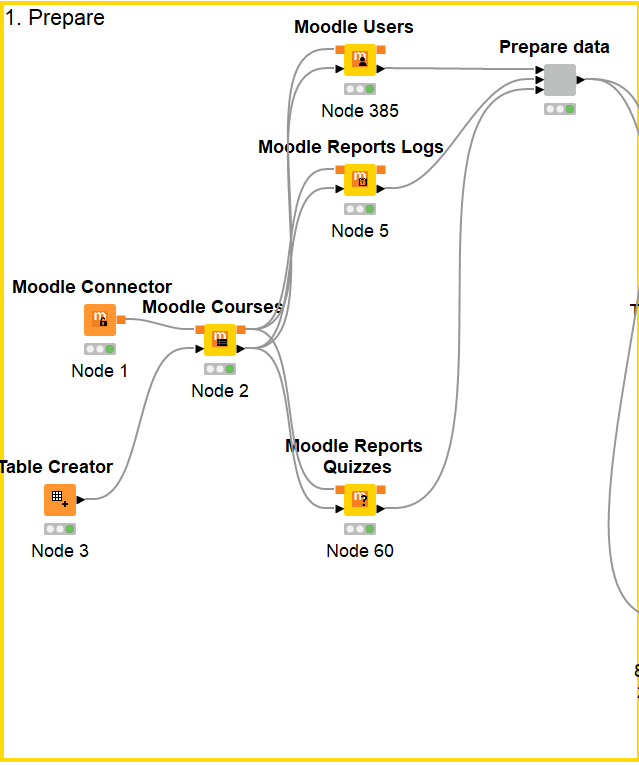
\includegraphics[width=1\textwidth]{img/workflow0.png}
	\caption{Workflow: preparación de datos}
	\label{fig:workflow0}
\end{figure}
\FloatBarrier

Si desplegamos el componente Prepare data, veremos componentes adicionales para la extracción y tratamiento de datos específicos (Figura ~\ref{fig:workflow1}): 

\begin{figure}[!htb]
	\centering
	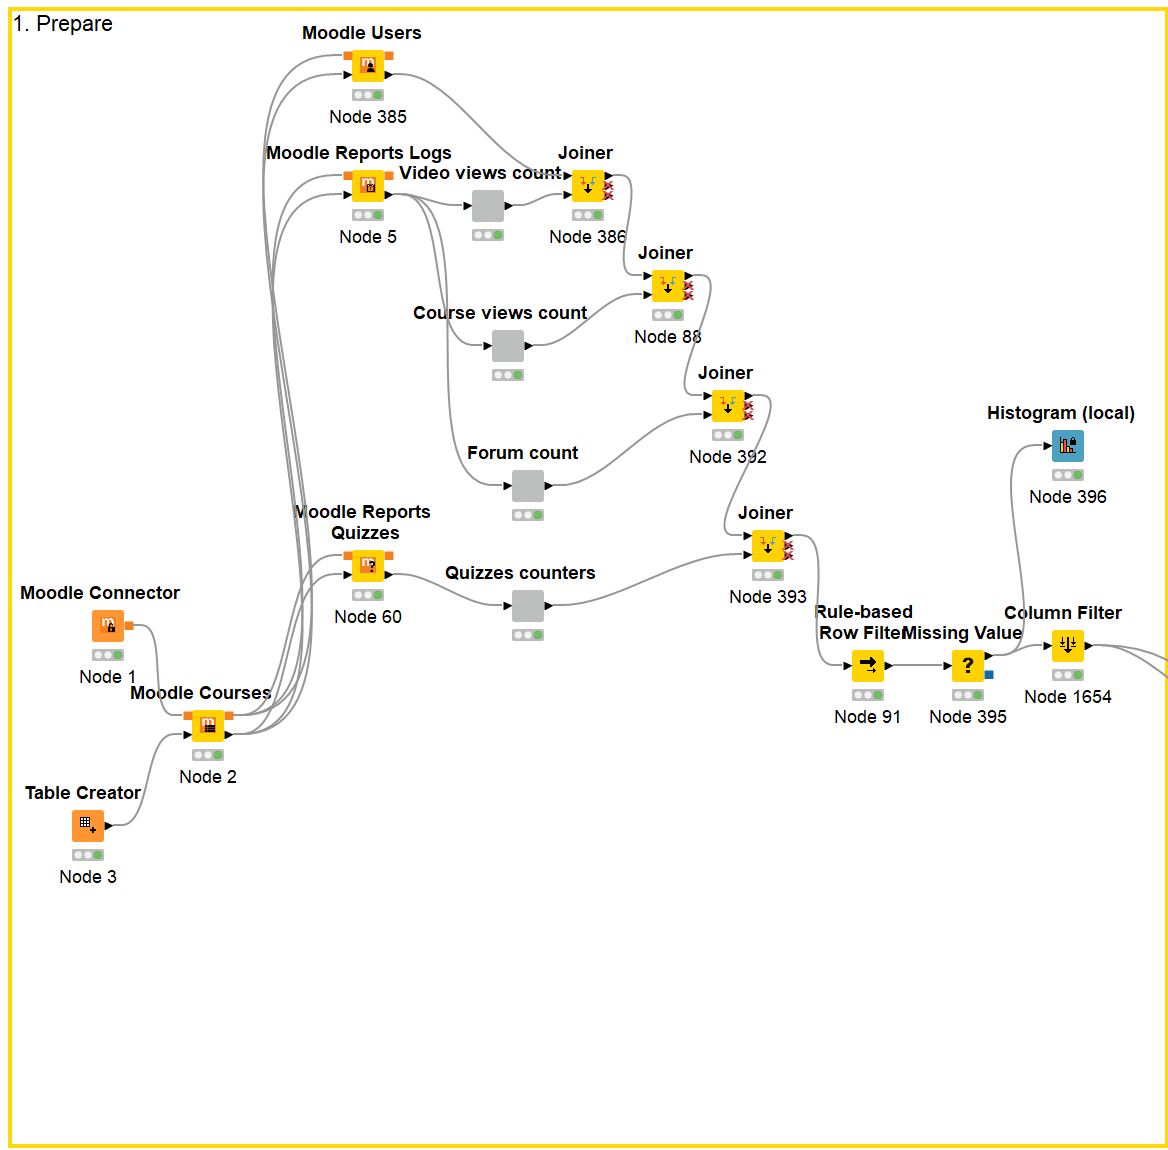
\includegraphics[width=1\textwidth]{img/workflow1.png}
	\caption{Workflow: preparación de datos (Prepare data desplegado)}
	\label{fig:workflow1}
\end{figure}
\FloatBarrier

El componente \textbf{Video View Count} ~\ref{fig:workflow1a} obtiene los datos de log desde el nodo \textbf{Moodle Reports Logs} y filtra aquellos
logs relacionados con la visualización de vídeos. Utilizando un nodo \textbf{GroupBy} realiza un conteo agrupando por curso y usuario, devolviendo el campo \textbf{videosviews}.

\begin{figure}[!htb]
	\centering
	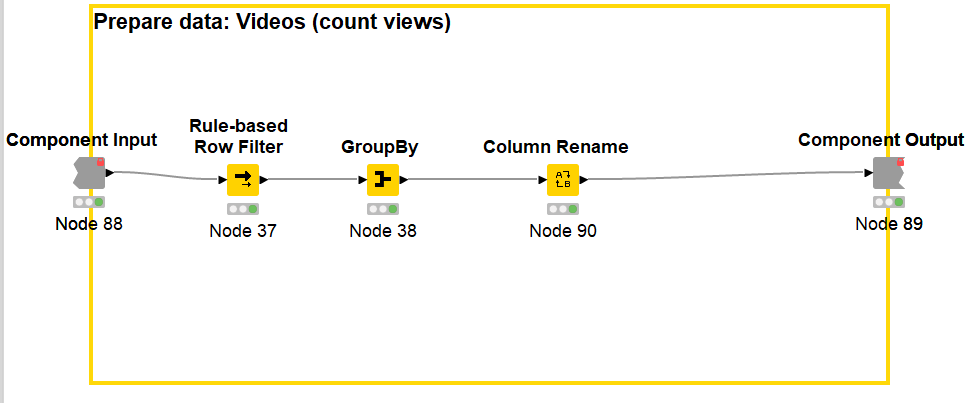
\includegraphics[width=1\textwidth]{img/workflow1a.png}
	\caption{Workflow: componente Video views count}
	\label{fig:workflow1a}
\end{figure}
\FloatBarrier

Los componentes \textbf{Course views count} y \textbf{Forum count} funcionan de forma similar al anterior pero filtrando por los logs correspondientes a cada caso y 
devolviendo los campos \textbf{courseviews} y \textbf{forumcount} respectivamente. 

El componente \textbf{Quizzes counters} obtiene, a partir del nodo \textbf{Moodle Reports Quizzies}, información de los intentos de cuestionarios 
realizados por los usuarios y agrupa los resultados para obtener los otros campos que necesitamos \textbf{autoevaltotalattempts}, \textbf{autoevalgrademean} y la clase, \textbf{evalgradecategory}.

Se han realizado las siguientes operaciones de preparación y limpieza de los datos: 

\begin{itemize}
	\item Los valores nulos en calificaciones se han considerado 0. 
	\item Se han eliminado los usuarios que no han realizado ningún cuestionario de evaluación.
\end{itemize}

Tras la limpieza de datos, nos hemos quedado con un conjunto de 53 registros. En la Figura ~\ref{fig:workflow2} se muestra un fragmento de la tabla de salida con las variables necesarias para el estudio. 

\begin{figure}[!htb]
	\centering
	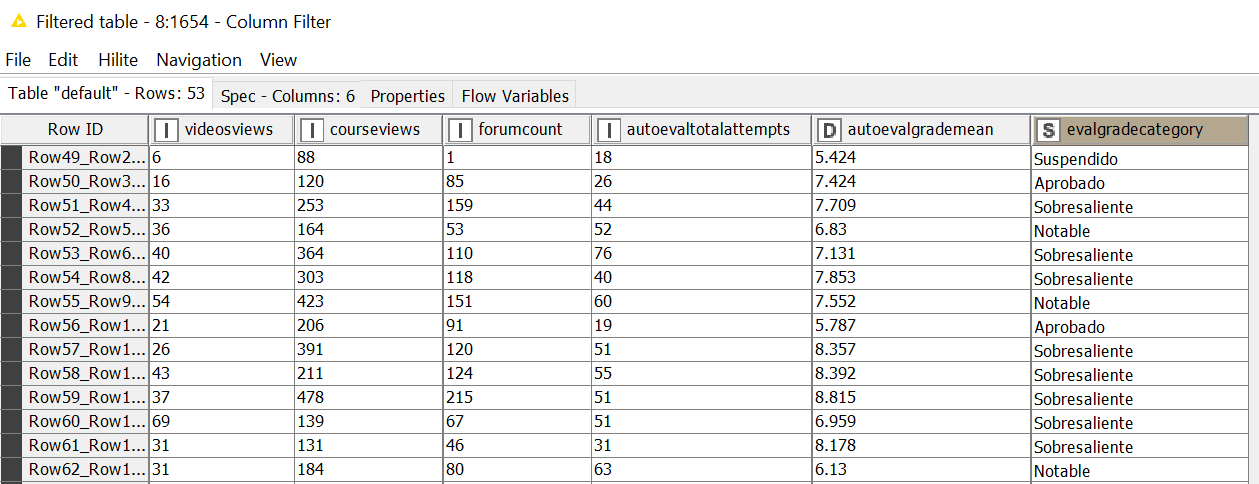
\includegraphics[width=1\textwidth]{img/workflow2.png}
	\caption{Workflow: preparación de datos (salida)}
	\label{fig:workflow2}
\end{figure}
\FloatBarrier

Como la clase es una variable cualitativa nominal, mostramos un diagrama de barras (Figura ~\ref{fig:workflow3}) con la frecuencia de cada valor posible de calificación (Suspendido, Aprobado, Notable y Sobresaliente). 

\begin{figure}[!htb]
	\centering
	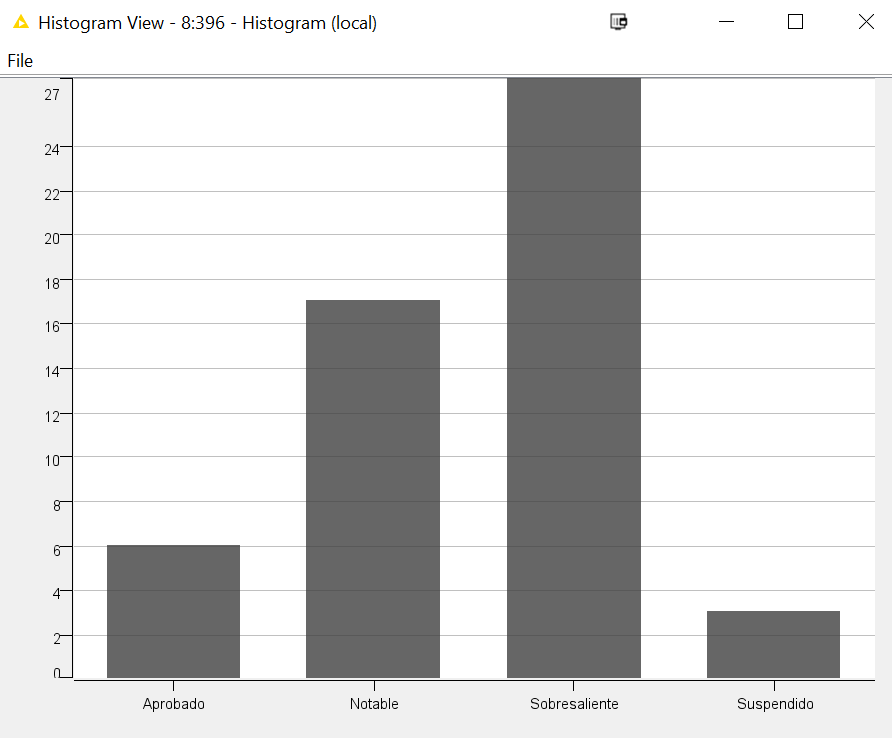
\includegraphics[width=1\textwidth]{img/workflow3.png}
	\caption{Workflow: preparación de datos (diagrama de barras clase)}
	\label{fig:workflow3}
\end{figure}
\FloatBarrier


\subsection{Modelo de aprendizaje}

En la Figura ~\ref{fig:workflow4} se muestra el workflow completo. Se han implementando tres variantes del modelo con el mismo 
objetivo, identificadas como Modelo A, Modelo B y Modelo C. 

\begin{figure}[!htb]
	\centering
	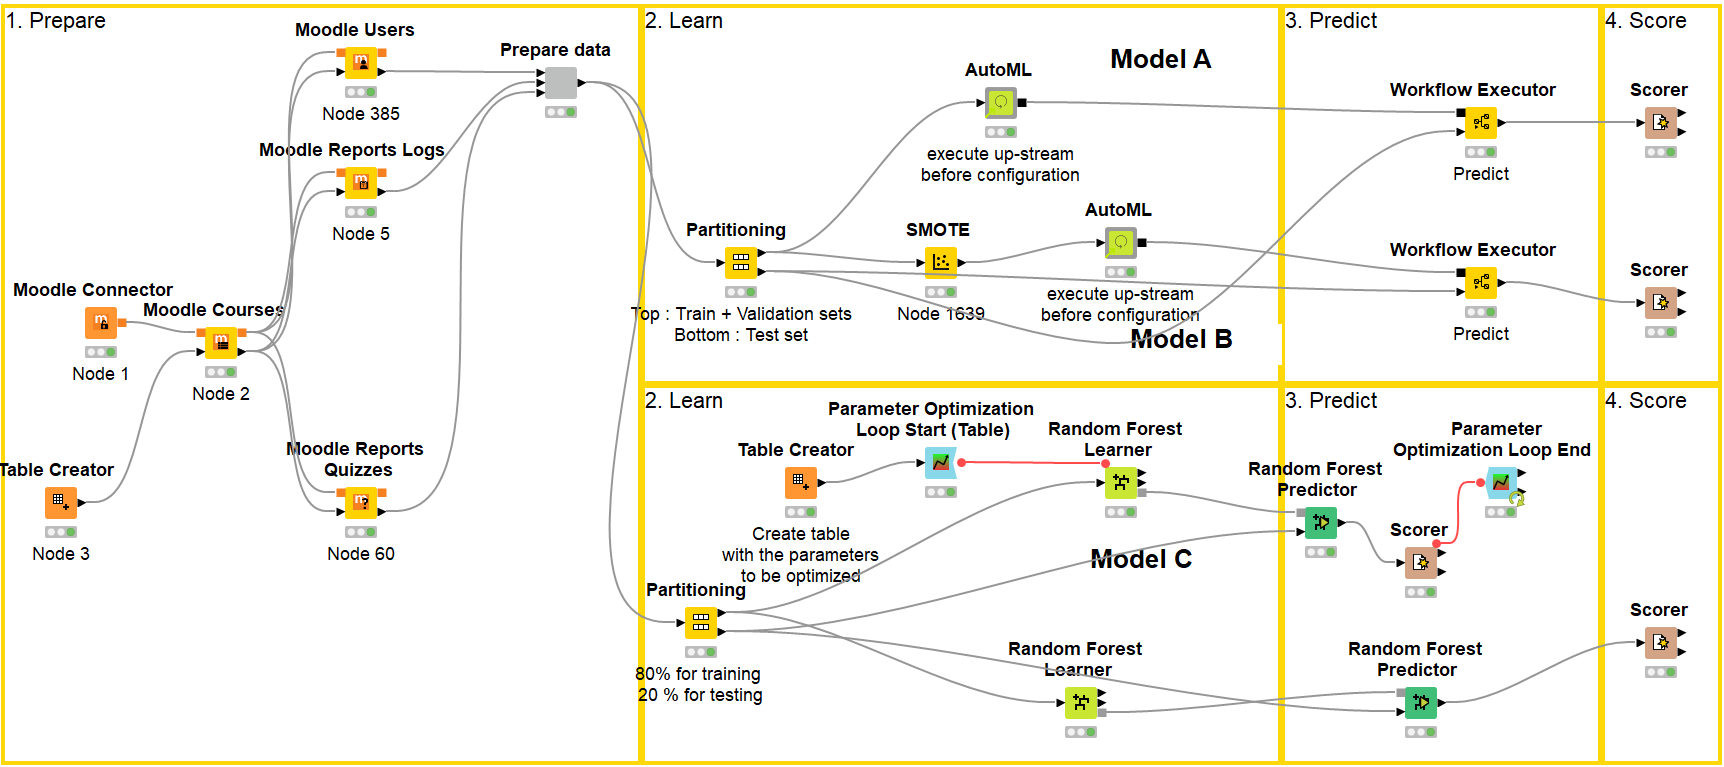
\includegraphics[width=1\textwidth]{img/workflow4.png}
	\caption{Workflow completo}
	\label{fig:workflow4}
\end{figure}
\FloatBarrier

\subsubsection{Modelo A}

En el modelo A, mostrado en la Figura ~\ref{fig:workflowA1} utilizamos el componente \textbf{AutoML} de KNIME. Este componente entrena automáticamente modelos 
de aprendizaje automático supervisados para clasificación binaria o multiclase, siendo este segundo nuestro objetivo. 

El componente incluye y automatiza todo el ciclo de Machine Learning, incluyendo preparación de datos, optimización 
de parámetros con validación cruzada y evaluación y selección del mejor modelo. 

\begin{figure}[!htb]
	\centering
	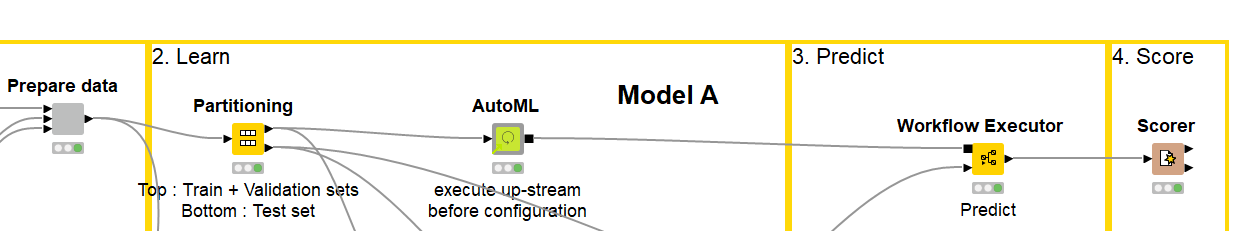
\includegraphics[width=1\textwidth]{img/workflowA1.png}
	\caption{Modelo A: Workflow}
	\label{fig:workflowA1}
\end{figure}
\FloatBarrier

No tenemos que ver AutoML como una caja cerrada que lo hace todo por nosotros. Lo interesante está en el hecho de que 
AutoML se ha construido como un componente y no como un nodo, con lo que realmente se trata de un workflow más complejo 
que se ha agrupado como componente. Este componente puede ser expandido y podemos visualizar sus elementos y modificarlos 
según las necesidades del proyecto. En la Figura ~\ref{fig:workflowA3} se muestra el primer nivel de expansión del componente,
que a su vez está formado por otros componetes que también se pueden abrir. 

\begin{figure}[!htb]
	\centering
	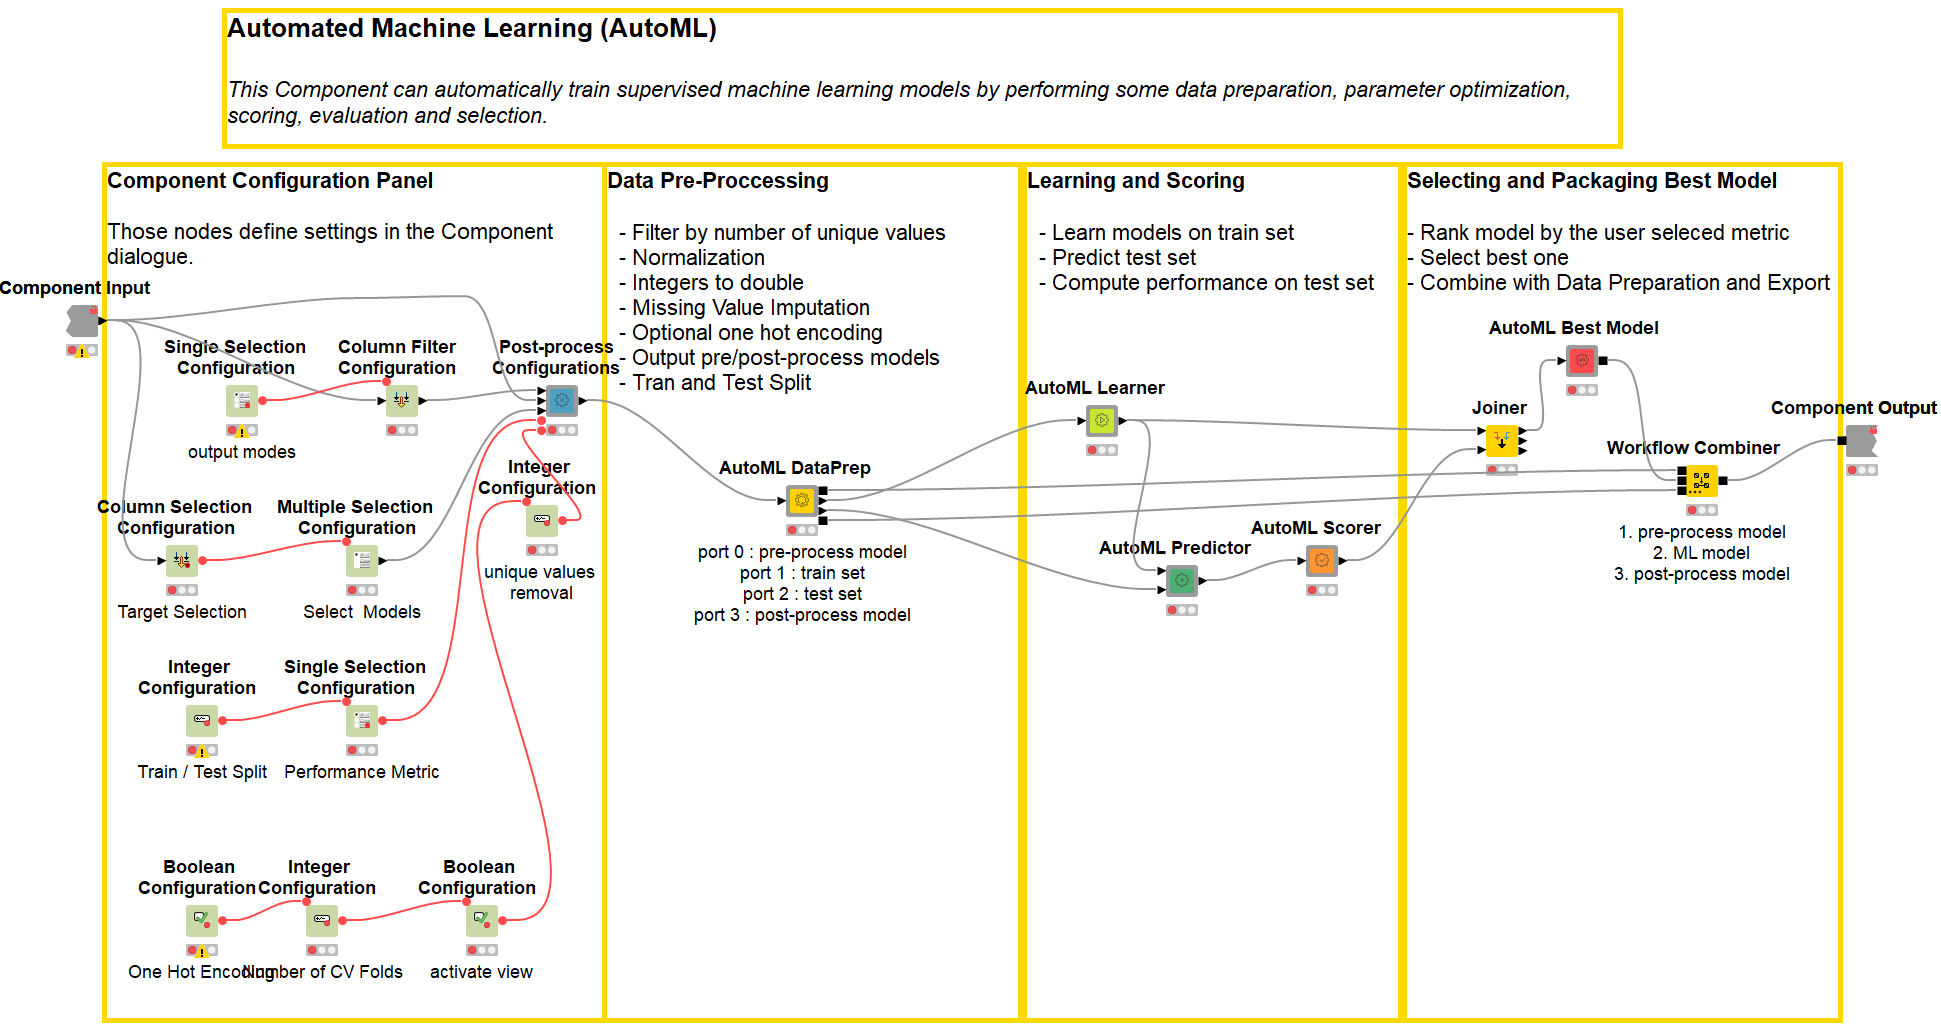
\includegraphics[width=1\textwidth]{img/workflowA3.png}
	\caption{Modelo A: Componente AutoML expandido}
	\label{fig:workflowA3}
\end{figure}
\FloatBarrier

En la Figura ~\ref{fig:workflowA2} se muestra la configuración del componente AutoML para nuestro modelo, donde hemos seleccionado los 
modelos a entrenar: 

\begin{itemize}
	\item Naive Bayes
	\item Logistic Regression
	\item Gradient Boosted Trees 
	\item Decision Tree 
	\item Random Forest 
	\item XGBoost Trees
\end{itemize}

\begin{figure}[!htb]
	\centering
	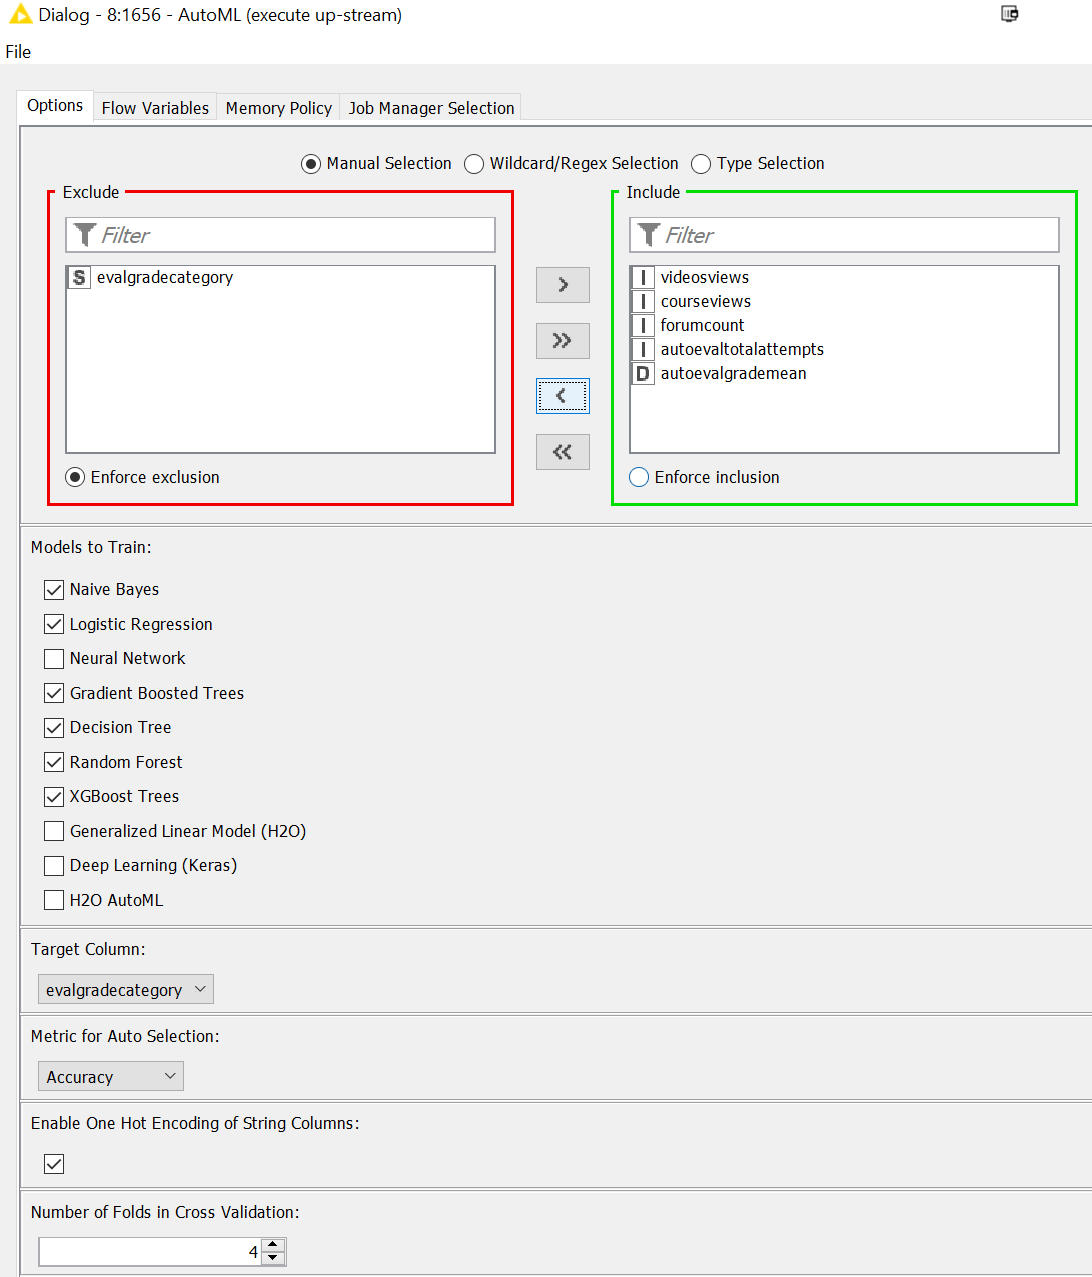
\includegraphics[width=1\textwidth]{img/workflowA2.png}
	\caption{Modelo A: Componente AutoML configuración}
	\label{fig:workflowA2}
\end{figure}
\FloatBarrier

Como resultado de la ejecución, AutoML nos muestra un listado de los modelos ordenados por Accuracy (Figura ~\ref{fig:workflowA4}). 
Los modelos Gradient Boosted Trees, Logistic Regression, Decision Tree y Random Forest obtienen los valores más altos (Accuracy = 0.67)

\begin{figure}[!htb]
	\centering
	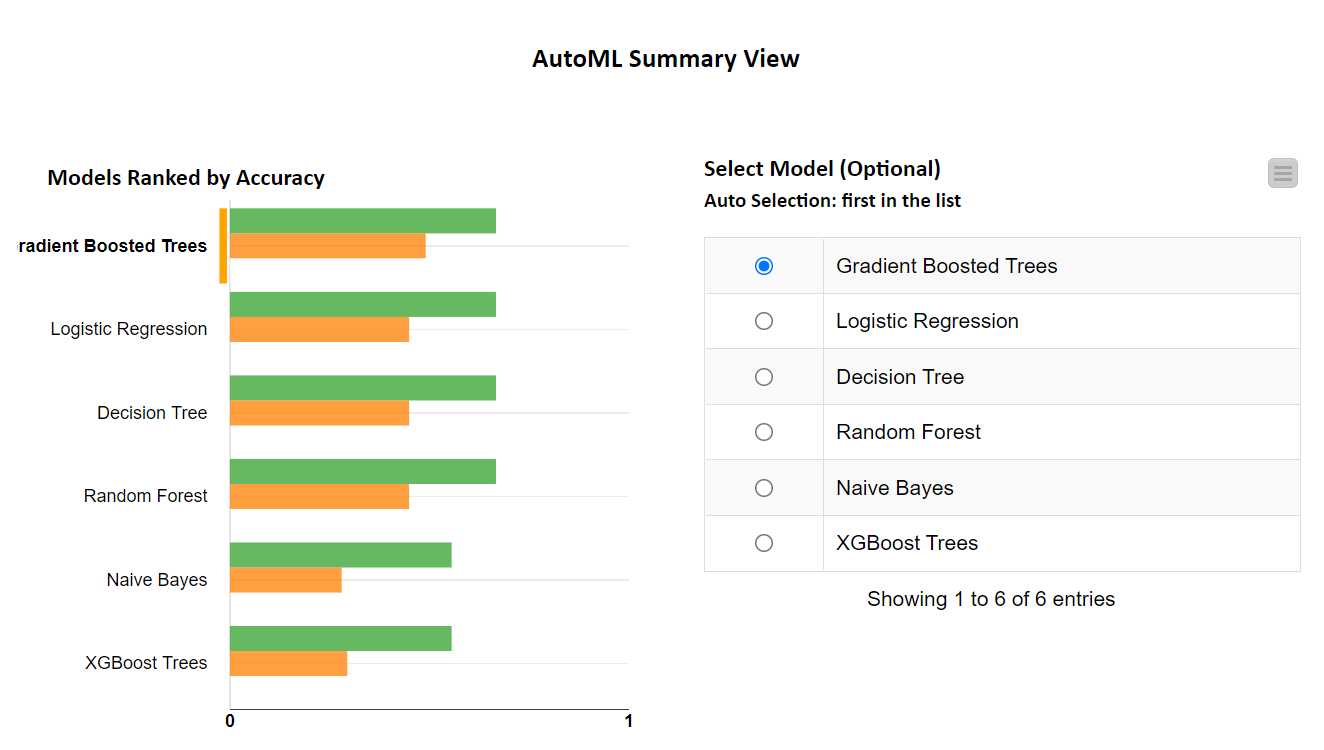
\includegraphics[width=1\textwidth]{img/workflowA4.png}
	\caption{Modelo A: Resultados}
	\label{fig:workflowA4}
\end{figure}
\FloatBarrier

\subsubsection{Modelo B}

El modelo B (Figura ~\ref{fig:workflowB1}) es una variante del anterior, usando también AutoML, pero añadiendo previamente sobremuestreo a los datos 
de entrada para enriquecer los datos de entrenamiento e igualar la distribución de clases. Esta técnica se llama 
SMOTE \cite{smote} (Synthetic Minority Over-sampling Technique) y KNIME dispone de un nodo que la implementa y que hemos 
configurado para que relice un sobremuestreo de las clases minoritarias. Esta técnica ha sido utilizada en otros estudios similares de 
predicción de calificaciones de estudiantes \cite{multiclass-pred}. 

\begin{figure}[!htb]
	\centering
	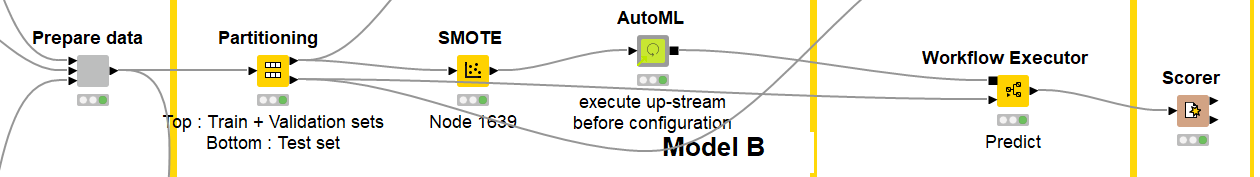
\includegraphics[width=1\textwidth]{img/workflowB1.png}
	\caption{Modelo B: Workflow}
	\label{fig:workflowB1}
\end{figure}
\FloatBarrier

La distribución de clases ahora se muestra en la Figura ~\ref{fig:workflowB2}

\begin{figure}[!htb]
	\centering
	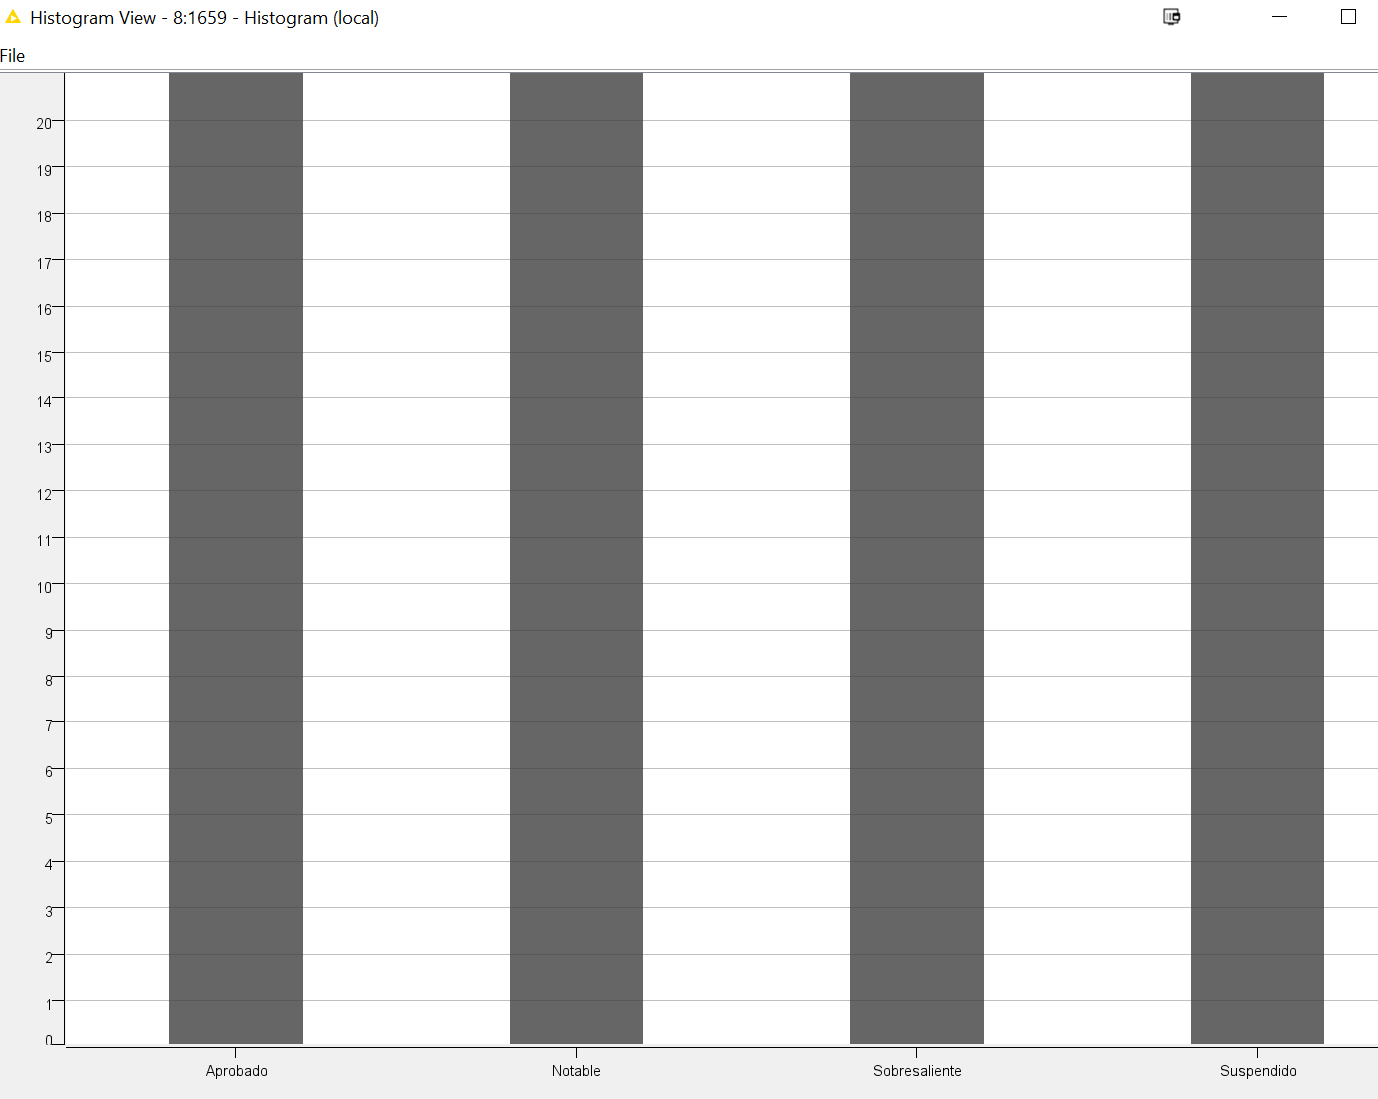
\includegraphics[width=1\textwidth]{img/workflowB2.png}
	\caption{Modelo B: SMOTE}
	\label{fig:workflowB2}
\end{figure}
\FloatBarrier

Como resultado, vemos que se obtiene un valor mayor de Accuracy (0.76) en todos los modelos a excepción de Naive Bayes. 

\begin{figure}[!htb]
	\centering
	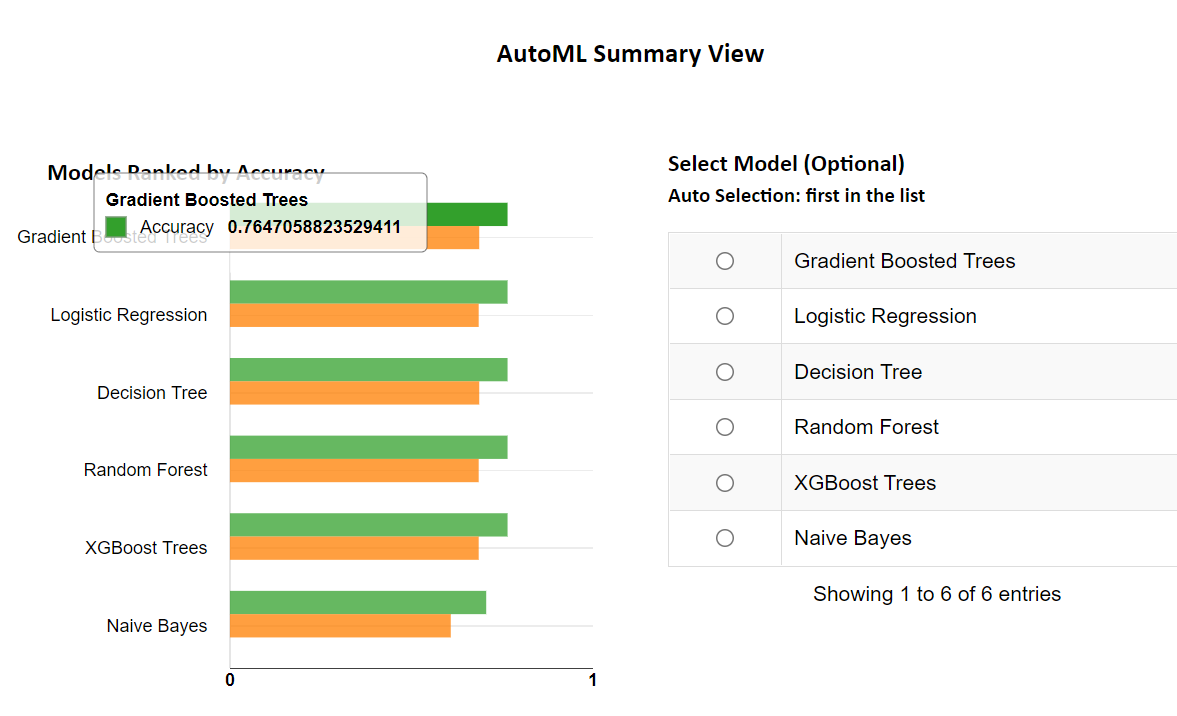
\includegraphics[width=1\textwidth]{img/workflowB3.png}
	\caption{Modelo B: Resultados}
	\label{fig:workflowB3}
\end{figure}
\FloatBarrier

\subsubsection{Modelo C}

En modelo C (Figura ~\ref{fig:workflowC1}) se entrena un modelo Random Forest con optimización de parámetros. 

\begin{figure}[!htb]
	\centering
	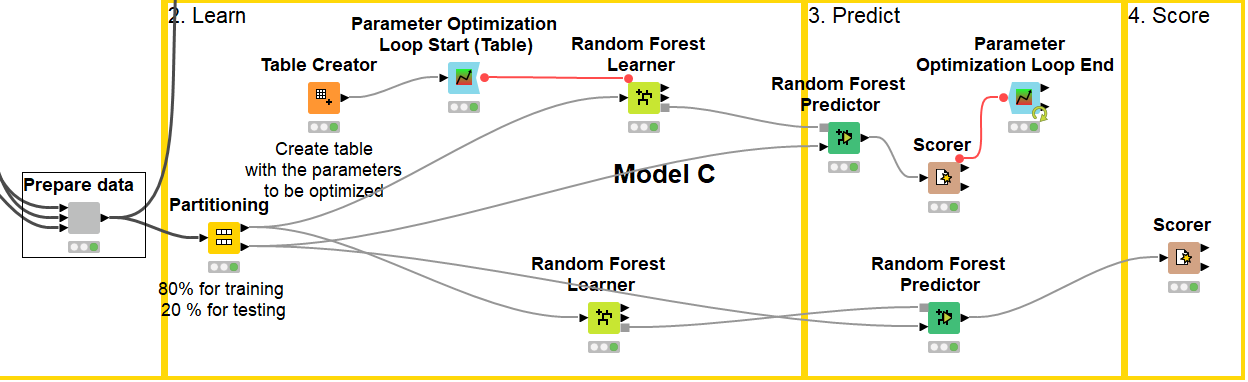
\includegraphics[width=1\textwidth]{img/workflowC1.png}
	\caption{Modelo C: Workflow}
	\label{fig:workflowC1}
\end{figure}
\FloatBarrier

En la parte superior se observa el flujo desarrollado para ejecutar el modelo con varios parámetros y seleccionar la combinación con la 
que se obtiene un mejor valor de Accuracy (Figura ~\ref{fig:workflowC2}). 

\begin{figure}[!htb]
	\centering
	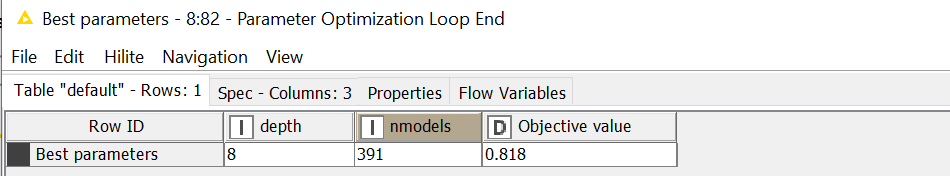
\includegraphics[width=1\textwidth]{img/workflowC2.png}
	\caption{Modelo C: Best parameters}
	\label{fig:workflowC2}
\end{figure}
\FloatBarrier

Estos parámetros se utilizarán para configurar el modelo y obtener el modelo final. En la Figura ~\ref{fig:workflowC3} se muestra
el valor de Accuracy de este modelo (0.818) y la tabla de confusión correspondiente. 

\begin{figure}[!htb]
	\centering
	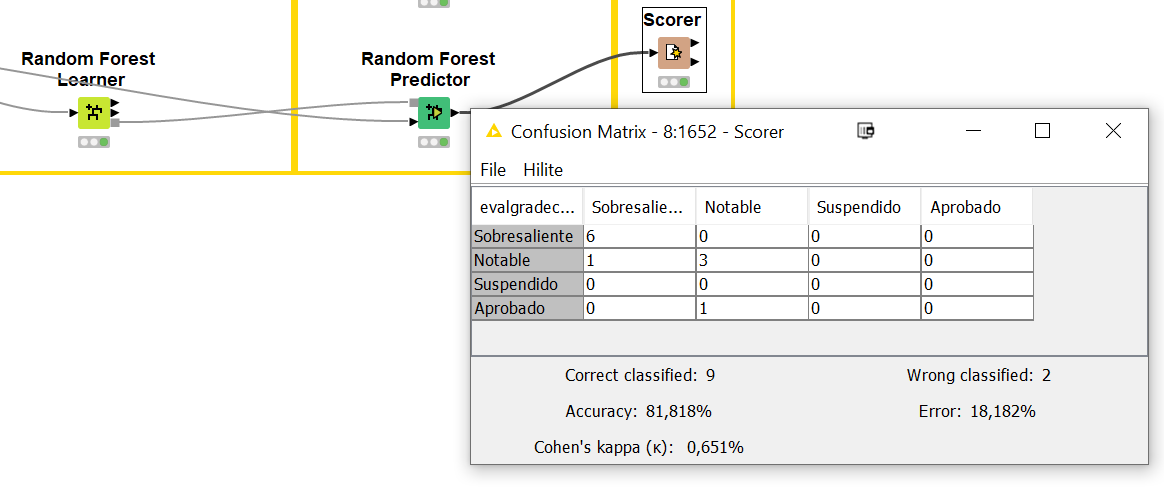
\includegraphics[width=1\textwidth]{img/workflowC3.png}
	\caption{Modelo C: Tabla de confusión}
	\label{fig:workflowC3}
\end{figure}
\FloatBarrier

